\documentclass[]{article}

\usepackage[utf8]{inputenc}

\usepackage[T1]{fontenc}

\usepackage[french]{babel}

\usepackage{amsmath, amsfonts, amssymb, amsthm}

\usepackage{fullpage}

\usepackage{enumerate}
\usepackage{graphicx}
\usepackage{algorithm}
\usepackage{algorithmic}

\usepackage{hyperref}
\hypersetup{
    colorlinks,
    citecolor=black,
    filecolor=black,
    linkcolor=black,
    urlcolor=black
}


%Pour les algos
\floatname{algorithm}{Algorithme}
\renewcommand{\algorithmicrequire}{\textbf{Entrée:}}
\renewcommand{\algorithmicensure}{\textbf{Sortie:}}
\renewcommand{\algorithmicif}{\textbf{si}}
\renewcommand{\algorithmicthen}{\textbf{alors}}
\renewcommand{\algorithmicelse}{\textbf{sinon}}

\title{
{\Huge Speaker classification project}\\
Signal processing\\
}

\author{
\textbf{Dell’Aria Doriano}
\and
\textbf{Goffaux Lionel}\\
}

\date{\today\\
Academic Year 2020-2021\\
Bachelor's degree in Computer Science\\}

\begin{document}

\maketitle
\pagebreak

% \tableofcontents
% \pagebreak

\section{Introduction}
In this project, we are going to extract features of a set of voice samples, to be able to classify if the sample is a
male or female voice.

\section{Energy}
In the \autoref{energy}, we plot the sample and its energy. We observe that with a threshold of 5,
we are able to classify the voiced and unvoiced frames.
Then we use these voiced frames to extract all the features we need.


\begin{figure}[h]
    \centering
    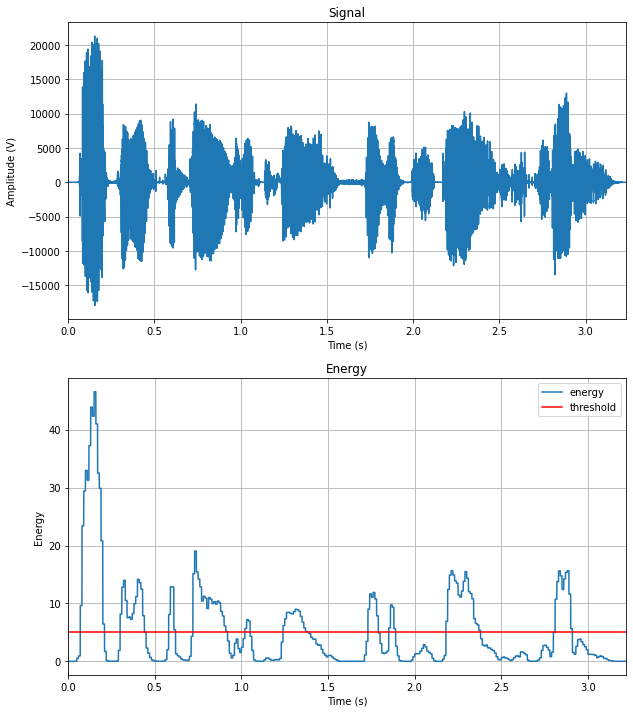
\includegraphics[scale=0.5]{images/energy_threshold.png}
    \caption{\label{energy}Energy of a sample}
\end{figure}

\section{Features extraction}
\subsection{Pitch}
They are multiple ways to exctract the pitch of a sample. In our case, we extract the pitch with an autocorrelation-based
system and a cepstrum-based system.

\subsubsection{autocorrelation}
The principle of autocorrelation is to correlate the signal with itself. We first split the signal into frames then autocorrelate
frames with themself.
So we obtain the pitch by measuring the distance between the distance of two peaks of the autocorrelation. 
we fix the frames width = 21, the step = 5 and the threshold = 5. 
In the \autoref{autocorr}, we observe that the method doesn't have 100\% accuracy because we obtain pitch over 5000 Hz.

\begin{figure}[h]
    \centering
    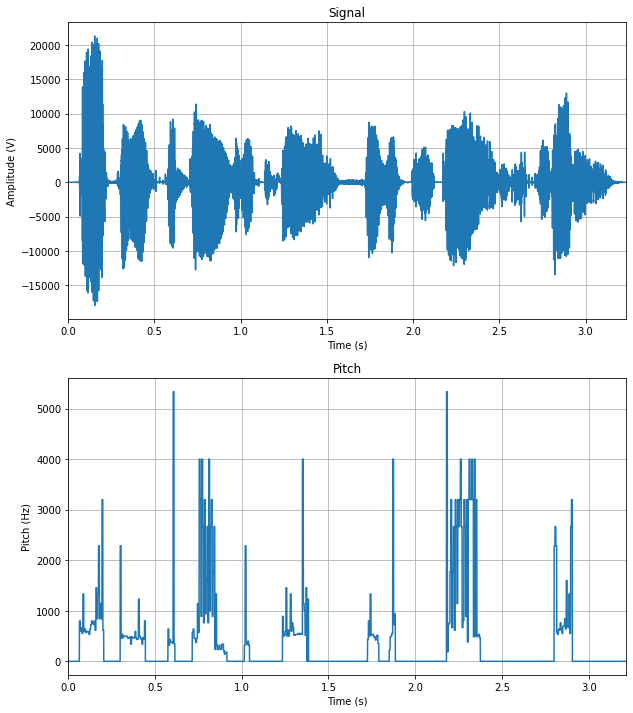
\includegraphics[scale=0.5]{images/autocorr_pitch.png}
    \caption{\label{autocorr}autocorrelation-based system}
\end{figure}

\subsubsection{Cepstrum}
test

\begin{figure}[h]
    \centering
    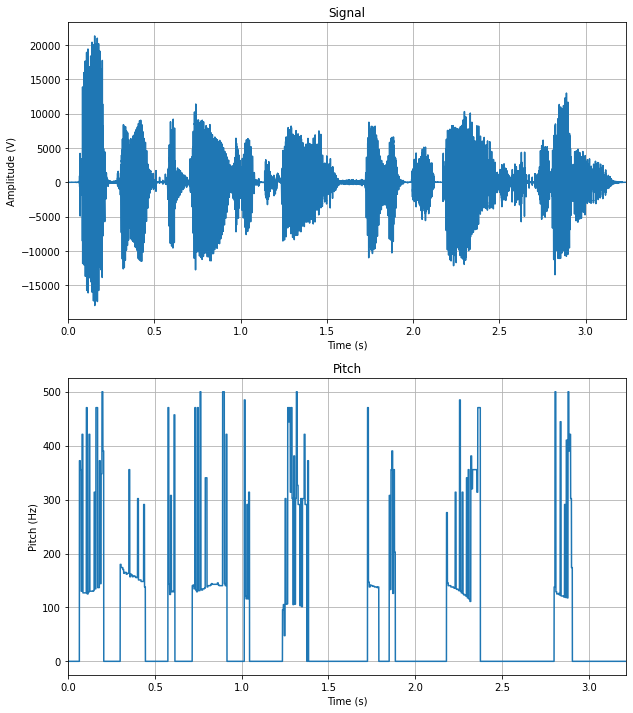
\includegraphics[scale=0.5]{images/cepstrum_pitch.png}
    \caption{\label{cepstrum}cepstrum-based system}
\end{figure}

\subsection{Formants}


\subsection{MFCC}




% ====== exemple d'algo =======
% \begin{algorithm}
%     \caption{Recherche linéaire du maximum}
%     \begin{algorithmic}[1]
%     \REQUIRE un tableau d’entiers $A$
%     \ENSURE la valeur du plus grand entier contenu dans $A$
%     \STATE $max \leftarrow -\infty$
%     \FOR{$i \leftarrow 1$ `a $longueur[A]$}
%     \IF{$max < A[i]$}
%     \STATE $max \leftarrow A[i]$
%     \ENDIF
%     \ENDFOR
%     \RETURN $max$
%     \end{algorithmic}
% \end{algorithm}


\end{document}